\problemname{House of Cards}

\illustration{0.3}{castle}{\href{https://commons.wikimedia.org/wiki/File:Card_castle6.JPG}{Picture} by Liftarn on Wikipedia, public domain}%
Brian and Susan are old friends, and they always dare each other to do
reckless things.  Recently Brian had the audacity to take the bottom
right exit out of their annual maze race, instead of the usual top
left one.  In order to trump this, Susan needs to think big.  She will
build a house of cards so big that, should it topple over, the entire
country would be buried by cards.  It's going to be huge!

The house will have a triangular shape.  The illustration to the right
shows a house of height $6$, and Figure~\ref{fig:house of cards} shows a schematic figure of a house of height $5$.

For aesthetic reasons, the cards used to build the tower should
feature each of the four suits (clubs, diamonds, hearts, spades)
equally often.  Depending on the height of the tower, this may or may
not be possible.  Given a lower bound $h_0$ on the height of the
tower, what is the smallest possible height $h \ge h_0$ such that it
is possible to build the tower?
\begin{figure}[h]
\centering
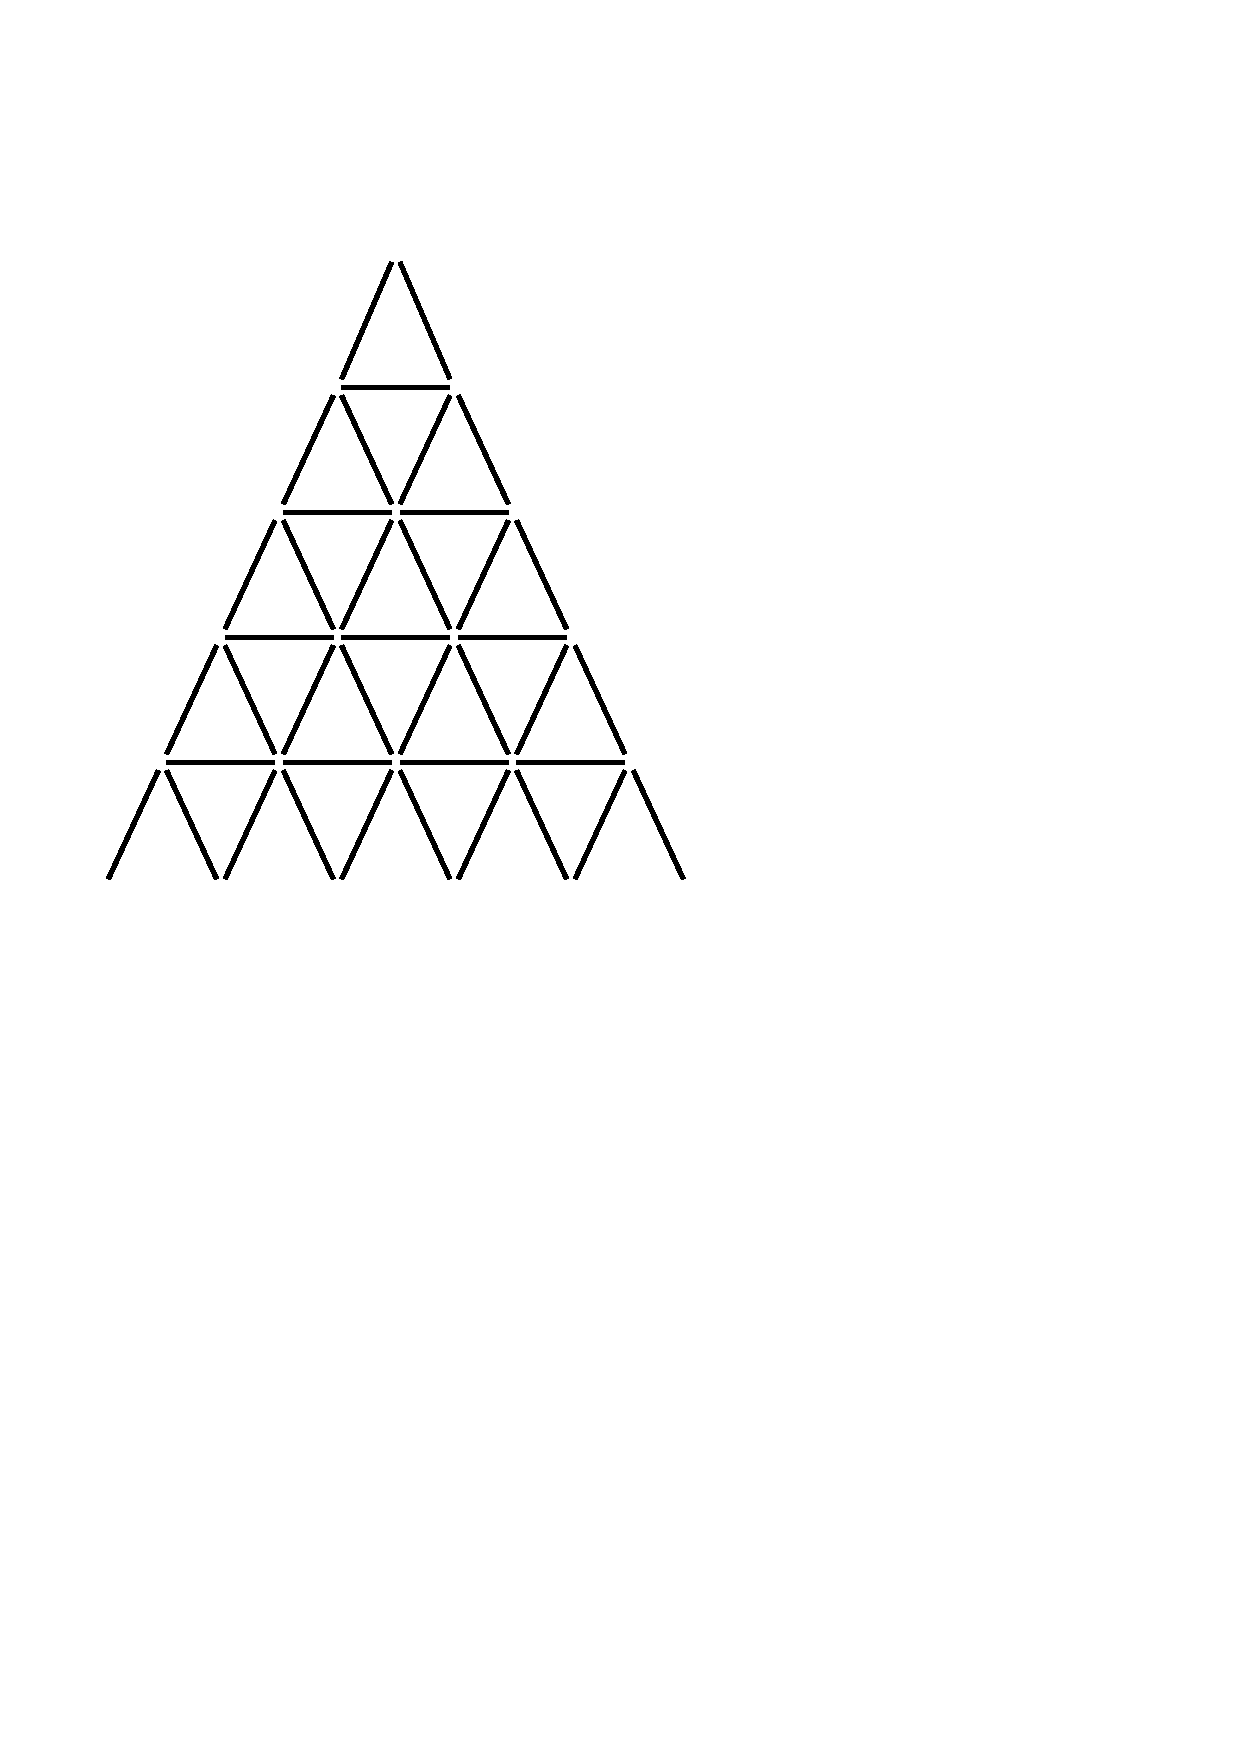
\includegraphics[width=0.25\textwidth]{fig}
\caption{A house of height $5$ uses $40$ cards.}
\label{fig:house of cards}
\end{figure}

\section*{Input}

A single integer $1 \le h_0 \le 10^{1000}$, the minimum height of the tower.

\section*{Output}

An integer, the smallest $h \ge h_0$ such that it is possible to build a tower of height $h$.
